\chapter{Implementasi dan Pengujian}
Pada bab ini, akan dibahas hasil dari implementasi perangkat lunak dan pengujian terhadap perangkat lunak. Pada tahap implementasi, terdapat spesifikasi lingkungan perangkat lunak yang digunakan. Spesifikasi ini juga digunakan pada tahap pengujian. Pada tahap pengujian, terdapat beberapa aspek yang diuji seperti pengujian terhadap fungsional perangkat lunak dan pengujian terhadap penyelesaian masalah.

\section{Lingkungan Implementasi dan Pengujian Perangkat Lunak}
Berikut ini merupakan spesifikasi yang digunakan pada saat implementasi dan pengujian perangkat lunak:
\begin{itemize}
	\item CPU: Intel\textsuperscript{\textregistered}{ }Core\texttrademark{ }i5-7200U Processor, 3M Cache, up to 3.10 Ghz
	\item GPU: NVIDIA GeForce 930MX
	\item RAM: 8GB
	\item OS: Windows 10 Pro, 64-bit
%	\item Compiler: Java SE Development Kit 8 Update 152 (64-bit)
%	\item Java Platform: Java 8 Update 152 (64-bit)
\end{itemize}

\section{Implementasi Antarmuka}
Pada bagian ini, akan dibahas hasil implementasi antarmuka berdasarkan perancangan antarmuka sebelumnya. Antarmuka diimplementasikan dengan menggunakan \textit{framework} antarmuka JavaFX yang disediakan oleh Java. Berikut ini merupakan hasil dari implementasi antarmuka:
\begin{itemize}
	\item Antarmuka: \textbf{Penerima Masukan}\\
	Pada gambar~\ref{fig:ui_input} dapat terlihat hasil implementasi antarmuka penerima masukan. Pada antarmuka ini terdapat kolom-kolom masukan yang dapat diisi oleh pengguna. Apabila sudah selesai diisi, pengguna dapat menekan tombol ''\textit{submit}''.
	\begin{figure}[H]
		\centering  
		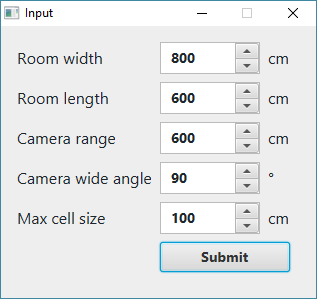
\includegraphics[scale=0.6]{ui_input}
		\caption[Antarmuka penerima masukan]{Antarmuka penerima masukan}
		\label{fig:ui_input}
	\end{figure}
	
	\item Antarmuka: \textbf{Simulasi Penempatan Kamera CCTV}\\
	Pada gambar~\ref{fig:ui_simulator} dapat terlihat hasil implementasi antarmuka simulasi penempatan kamera CCTV. Pada antarmuka ini, pengguna dapat melakukan simulasi penempatan kamera CCTV seperti dengan menempatkan kamera CCTV secara manual atau otomatis dan membuang suatu penempatan kamera CCTV. Pengguna dapat melihat visualisasi penempatan kamera CCTV melalui panel visualisasi yang berada di bagian kanan antarmuka. Informasi simulasi dan daftar penempatan kamera CCTV dapat dilihat pada panel informasi yang berada di bagian kiri antarmuka. Pada bagian kanan atas antarmuka terdapat panel penambah kamera CCTV yang digunakan untuk menambah penempatan kamera CCTV.
	\begin{figure}[H]
		\centering  
		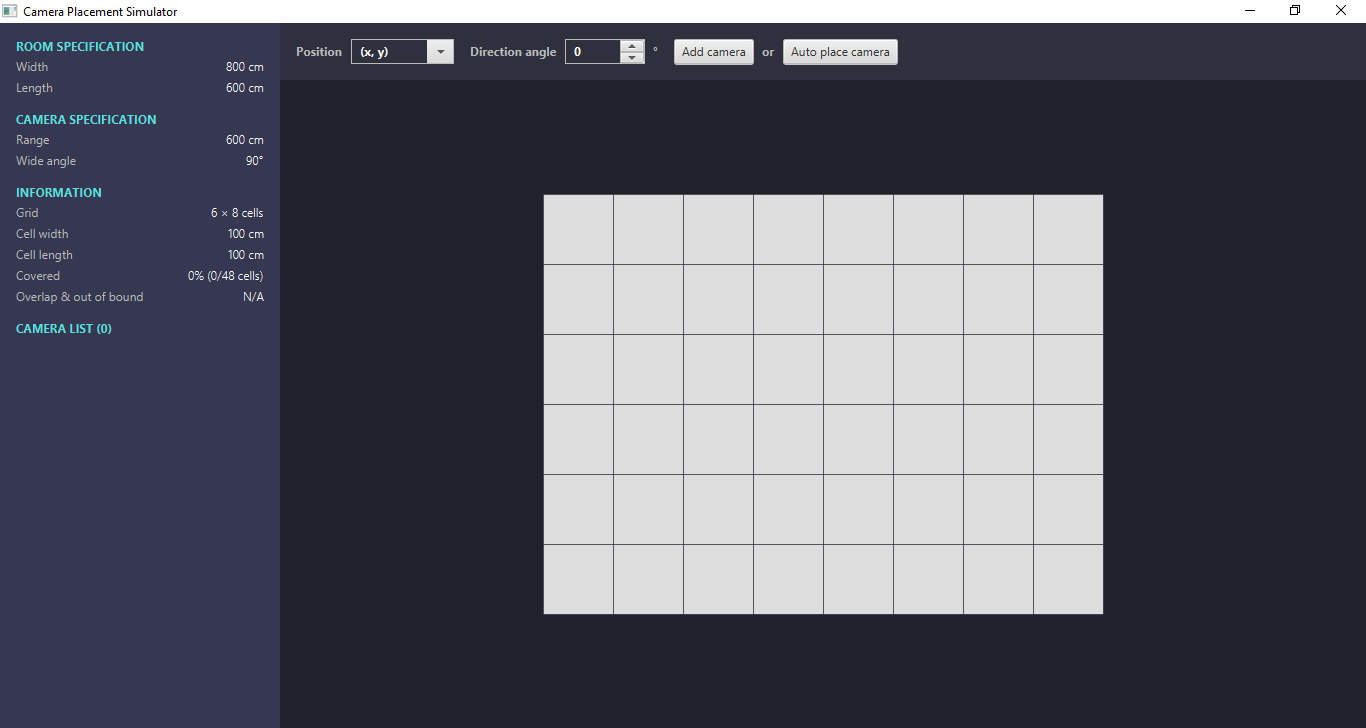
\includegraphics[scale=0.45]{ui_simulator}
		\caption[Antarmuka penempatan kamera CCTV]{Antarmuka penempatan kamera CCTV}
		\label{fig:ui_simulator}
	\end{figure}
\end{itemize}

\section{Pengujian Perangkat Lunak}
Perangkat lunak yang telah diimplementasikan perlu diuji terlebih dahulu agar berjalan sebagaimana mestinya. Pada bagian ini akan dibahas 2 jenis pengujian yang dilakukan, yaitu pengujian fungsional dan pengujian eksperimen. Pada pengujian fungsional, perangkat lunak akan diuji agar bekerja sesuai fungsinya. Pada pengujian eksperimen, akan diadakan beberapa eksperimen untuk mendapatkan hasil yang akan dianalisa.

\subsection{Pengujian Fungsional}
Pengujian yang terdapat pada pengujian fungsional dilakukan sesuai dengan skenario-skenario yang terdapat pada use case yang telah dibahas sebelumnya. Berikut ini pengujian-pengujian fungsional yang dilakukan:

\begin{itemize}
	\item Pengujian: \textbf{Memasukkan Spesifikasi Masalah}\\
	Pada pengujian ini akan diuji apakah perangkat lunak dapat membangun simulasi masalah yang sesuai dengan masukan yang diberikan oleh pengguna. Pengujian ini dimulai dengan mengisi masukan-masukan masalah melalui antarmuka penerima masukan. Berikut masukan-masukan masalah yang diisi melalui antarmuka penerima masukan seperti pada gambar~\ref{fig:testing_input_before}
	\begin{itemize}
		\item Lebar ruangan: 800cm
		\item Panjang ruangan: 600cm
		\item Jarak pandang kamera CCTV: 600cm
		\item Besar sudut pandang kamera CCTV: \(90^\circ\)
		\item Ukuran terbesar cell: 100cm
	\end{itemize}
	
	\begin{figure}[H]
		\centering  
		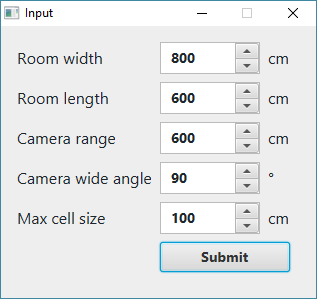
\includegraphics[scale=0.6]{ui_input}
		\caption[Tampilan pengisian masukan masalah]{Tampilan pengisian masukan masalah}
		\label{fig:testing_input_before}
	\end{figure}
	
	Setelah masukan-masukan tersebut diisi, tombol ''\textit{submit}'' ditekan. Perangkat lunak menampilkan antarmuka simulasi penempatan kamera CCTV seperti pada gambar~\ref{fig:testing_input_after}. 
	
	\begin{figure}[H]
		\centering  
		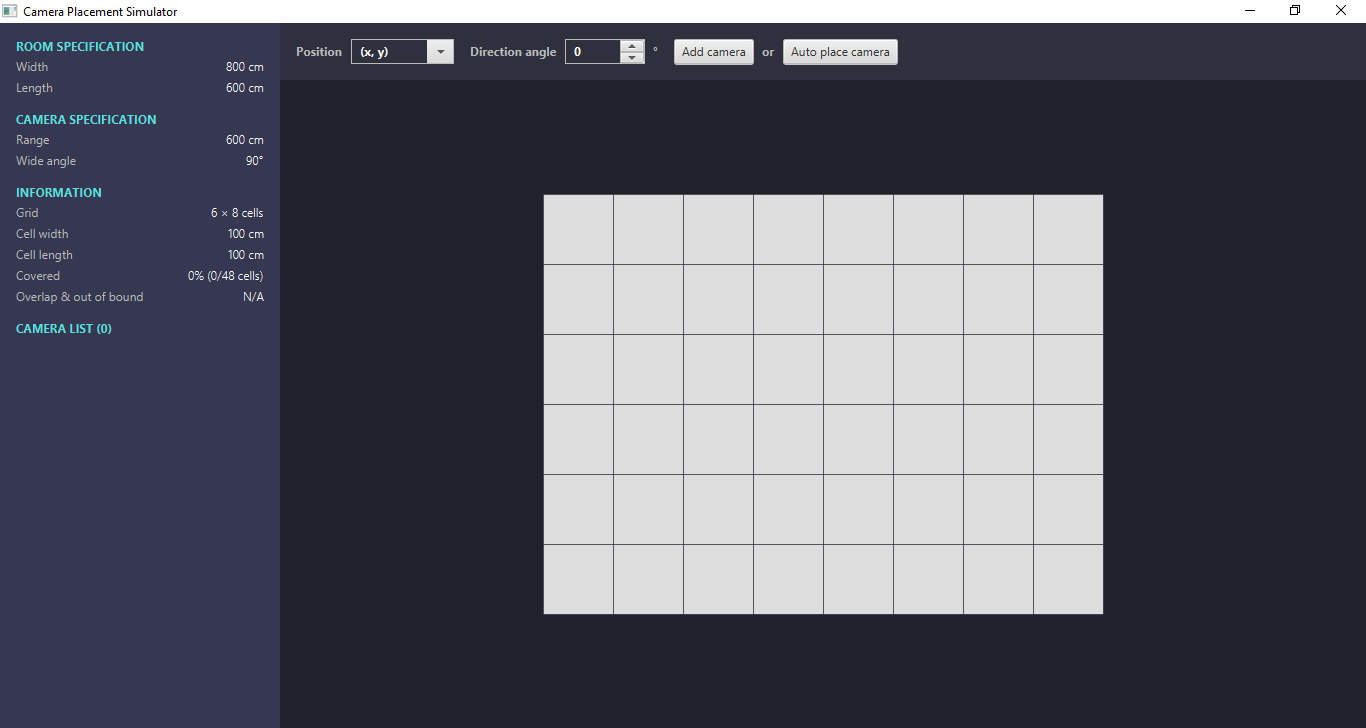
\includegraphics[scale=0.45]{ui_simulator}
		\caption[Tampilan setelah pengisian masukan masalah]{Tampilan setelah pengisian masukan masalah}
		\label{fig:testing_input_after}
	\end{figure}
	
	Pada gambar~\ref{fig:testing_input_side_pane_after} terdapat panel informasi yang menunjukkan informasi masalah yang sesuai dengan masukan diberikan sebelumnya. Hal ini menunjukkan bahwa proses memasukkan spesifikasi masalah telah berjalan sesuai dengan fungsinya. Dengan demikian, pengujian memasukkan spesifikasi masalah telah berhasil dilakukan.
	
	\begin{figure}[H]
		\centering  
		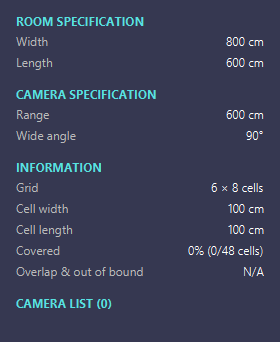
\includegraphics[scale=0.6]{testing_input_side_pane_after}
		\caption[Tampilan panel informasi setelah pengisian masukan masalah]{Tampilan panel informasi setelah pengisian masukan masalah}
		\label{fig:testing_input_side_pane_after}
	\end{figure}
	
	\item Pengujian: \textbf{Menambahkan Penempatan Kamera CCTV}\\
	Pada pengujian ini akan diuji apakah perangkat lunak dapat merespon penambahan penempatan kamera CCTV dengan memperbaharui panel informasi dan panel visualisasi penempatan kamera CCTV. Pengujian dilakukan dengan memilih koordinat (0, 0) sebagai posisi penempatan dan mengisi sudut (\(315^\circ\)) sebagai sudut arah pandang seperti pada gambar~\ref{fig:testing_add_placement_top_pane}.
	
	\begin{figure}[H]
		\centering  
		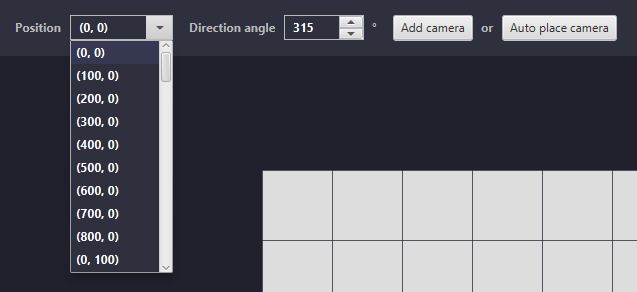
\includegraphics[scale=0.6]{testing_add_placement_top_pane}
		\caption[Tampilan panel penambahan penempatan kamera CCTV]{Tampilan panel penambahan penempatan kamera CCTV}
		\label{fig:testing_add_placement_top_pane}
	\end{figure}
	
	 Setelah mengisi informasi penempatan tersebut, tombol ''\textit{add camera}'' ditekan. Perangkat lunak merespon penambahan penempatan tersebut dengan memperbaharui panel informasi dan panel visualisasi seperti pada gambar~\ref{fig:testing_add_placement_side_pane_after} dan~\ref{fig:testing_add_placement_visualization_pane_after}. Proses menambahkan penempatan kamera CCTV telah berjalan sesuai dengan fungsinya. Dengan demikian, pengujian menambahkan penempatan kamera CCTV telah berhasil dilakukan.
	 
	 \begin{figure}[H]
		\centering  
		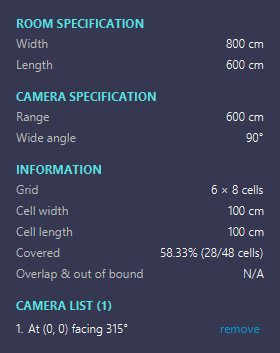
\includegraphics[scale=0.6]{testing_add_placement_side_pane_after}
		\caption[Tampilan panel informasi setelah menambah penempatan kamera CCTV]{Tampilan panel informasi setelah menambah penempatan kamera CCTV}
		\label{fig:testing_add_placement_side_pane_after}
	\end{figure}
	
	\begin{figure}[H]
		\centering  
		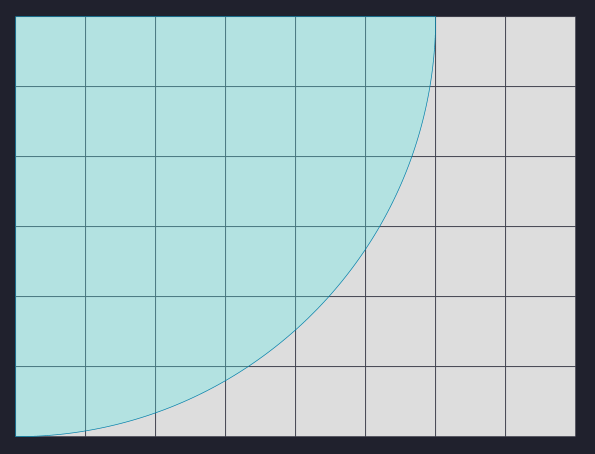
\includegraphics[scale=0.6]{testing_add_placement_visualization_pane_after}
		\caption[Tampilan panel visualisasi setelah menambah penempatan kamera CCTV]{Tampilan panel visualisasi setelah menambah penempatan kamera CCTV}
		\label{fig:testing_add_placement_visualization_pane_after}
	\end{figure}
	
	\item Pengujian: \textbf{Membuang Penempatan Kamera CCTV}\\
	Pada pengujian ini akan diuji apakah perangkat lunak dapat merespon pembuangan penempatan kamera CCTV dengan memperbaharui panel informasi dan panel visualisasi penempatan kamera CCTV. Pengujian dilakukan dengan memilih penempatan kamera CCTV yang akan dibuang. Penempatan kamera CCTV dipilih dari daftar penempatan kamera CCTV yang berada di dalam panel informasi. Pada pengujian ini, akan dipilih penempatan pada koordinat (0, 0) dengan sudut arah pandang (\(315^\circ\)) sebagai penempatan yang akan dibuang. Pada penempatan tersebut, tombol ''\textit{remove}'' ditekan. Perangkat lunak merespon pembuangan penempatan tersebut dengan memperbaharui panel informasi dan panel visualisasi seperti pada gambar~\ref{fig:testing_remove_placement_information_pane_after} dan~\ref{fig:testing_remove_placement_visualization_pane_after}. Proses membuang penempatan kamera CCTV telah berjalan sesuai dengan fungsinya. Dengan demikian, pengujian membuang penempatan kamera CCTV telah berhasil dilakukan.
	
	 \begin{figure}[H]
		\centering  
		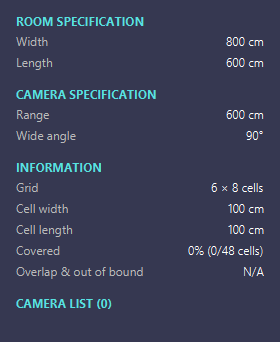
\includegraphics[scale=0.6]{testing_input_side_pane_after}
		\caption[Tampilan panel informasi setelah membuang penempatan kamera CCTV]{Tampilan panel informasi setelah membuang penempatan kamera CCTV}
		\label{fig:testing_remove_placement_information_pane_after}
	\end{figure}
	
	\begin{figure}[H]
		\centering  
		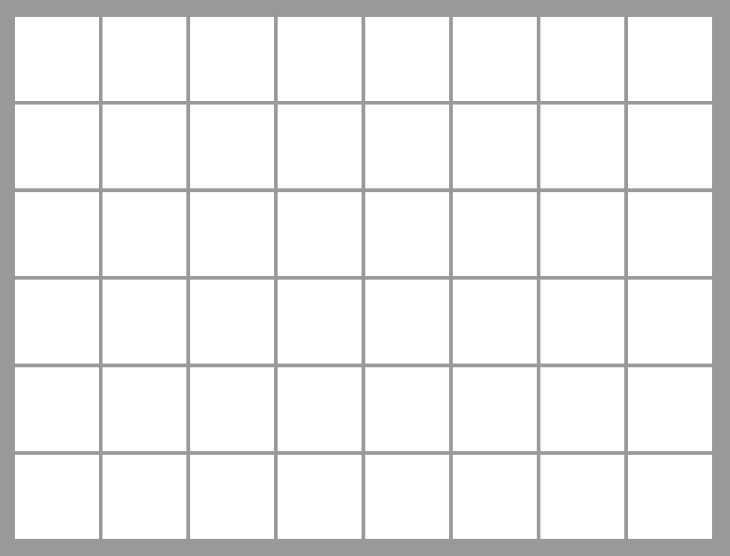
\includegraphics[scale=0.6]{testing_remove_placement_visualization_pane_after}
		\caption[Tampilan panel visualisasi setelah membuang penempatan kamera CCTV]{Tampilan panel visualisasi setelah membuang penempatan kamera CCTV}
		\label{fig:testing_remove_placement_visualization_pane_after}
	\end{figure}
\end{itemize}
